\documentclass{article}

\usepackage{hyperref}
\usepackage{graphicx}

\author{Nick Werle}
\title{P7 Submission}

\begin{document}
\maketitle
\section{Preamble}
This report's source files will be made available at \url{https://github.com/NickWer/CEG3900_P7}

\section{Task 1}
The user interface is okay. It seems really odd that it forced me to provide a username and password. Perhaps this is so users can track their contributions? Anyways other than that it seemed fine - nothing special.
My biggest critique of this app is probably just that - nothing special.
It's strange because there's no easy way to see just what work my phone did while charging, which makes me wonder what the traditional motivation is, outside of just a general sense of goodwill for furthering science.
In fact, opening the app does so little good that it actually has a bar at the bottom instructing you to just close the app and lock your phone - what good does that do me?

Anways, overall my impression of the app is that it's cool. It's cool at a technical level, in that it distributes workloads and solves tough problems.
On the other hand as a user, I can't really imagine wanting to install it - my experience as a user is that I just ignore it and each morning when I wake up my phone phone feels about as hot as molten lava.

If I could change something, I think it would be to provide some what to see what good my phone's effort actually has provided - just what, if anything, it was able to find/calculate.




\begin{figure}[ht]
      
\includegraphics[width=3in]{img/t1s1.png}
      \centering
      \caption{Landing screen}
\end{figure}
\begin{figure}[ht]
      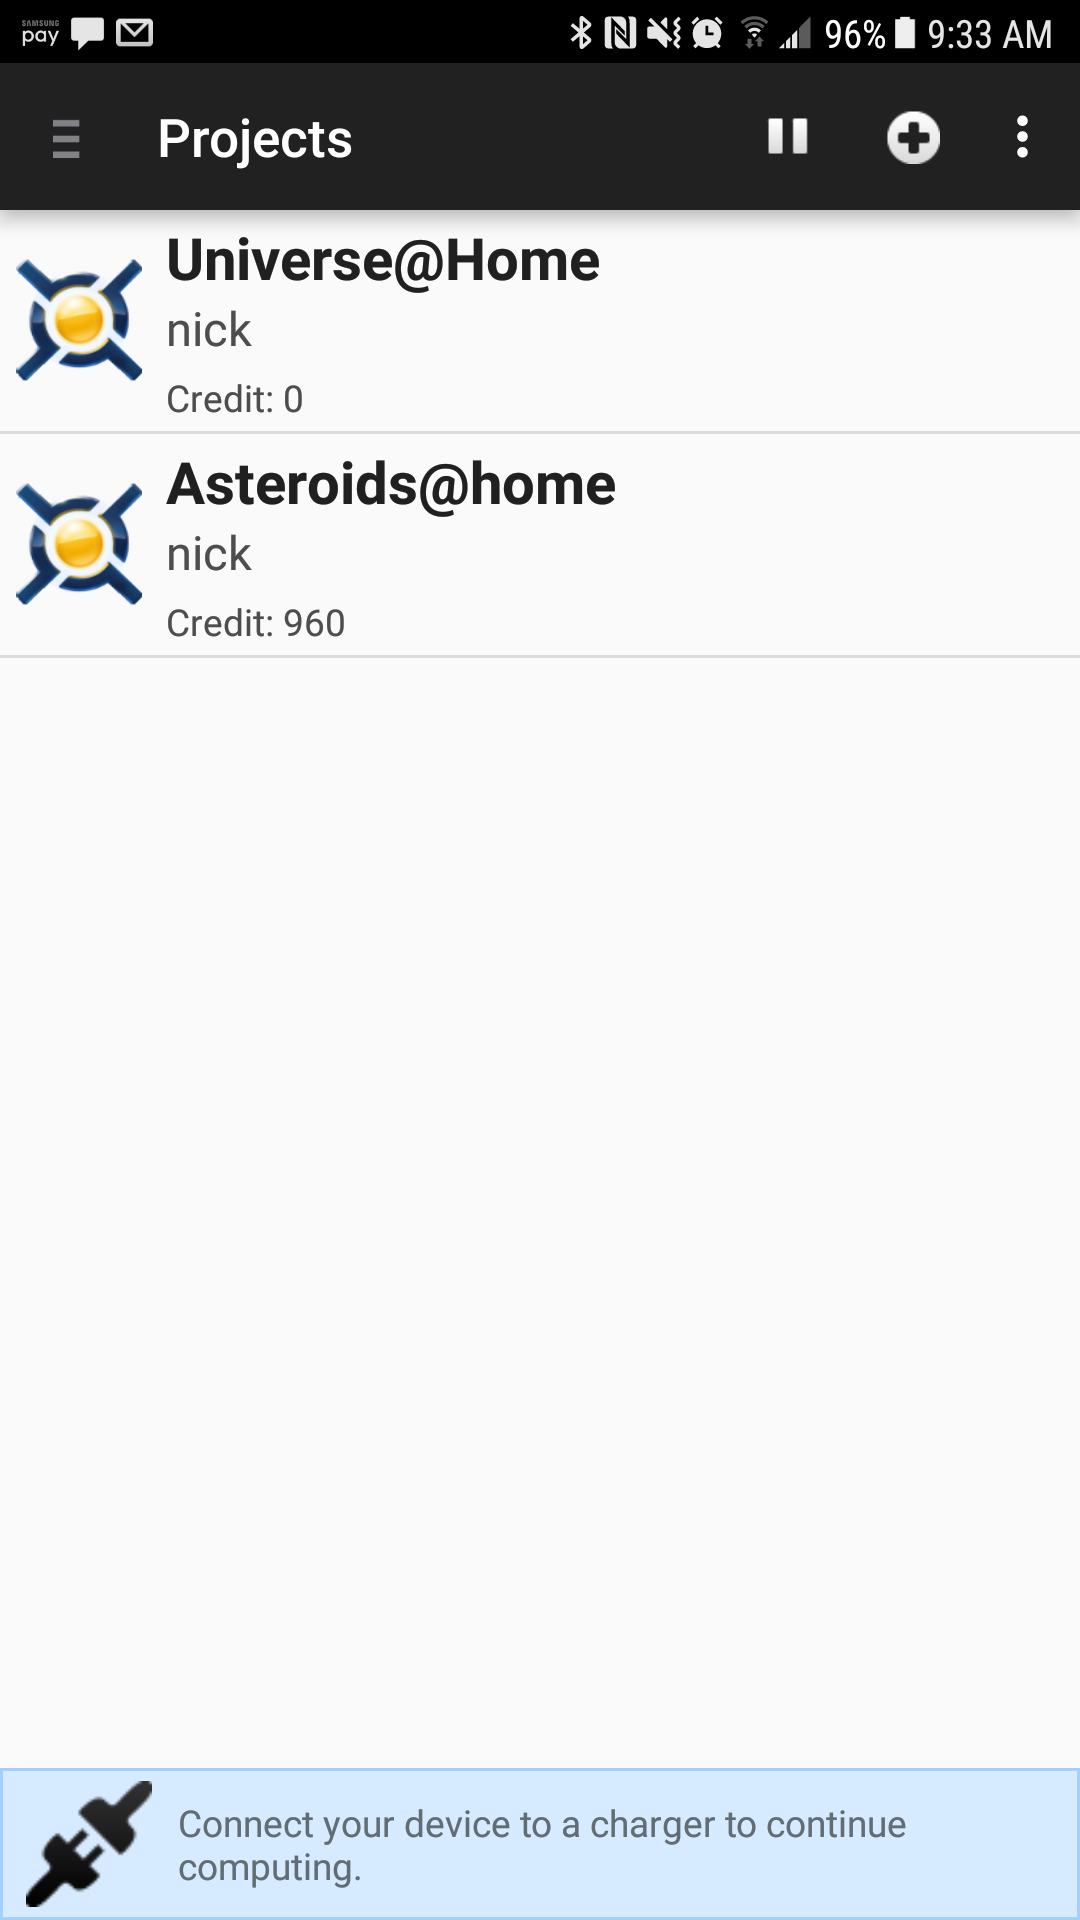
\includegraphics[width=3in]{img/t1s2.png}
      \centering
      \caption{Project List}
\end{figure}
\begin{figure}[ht]
      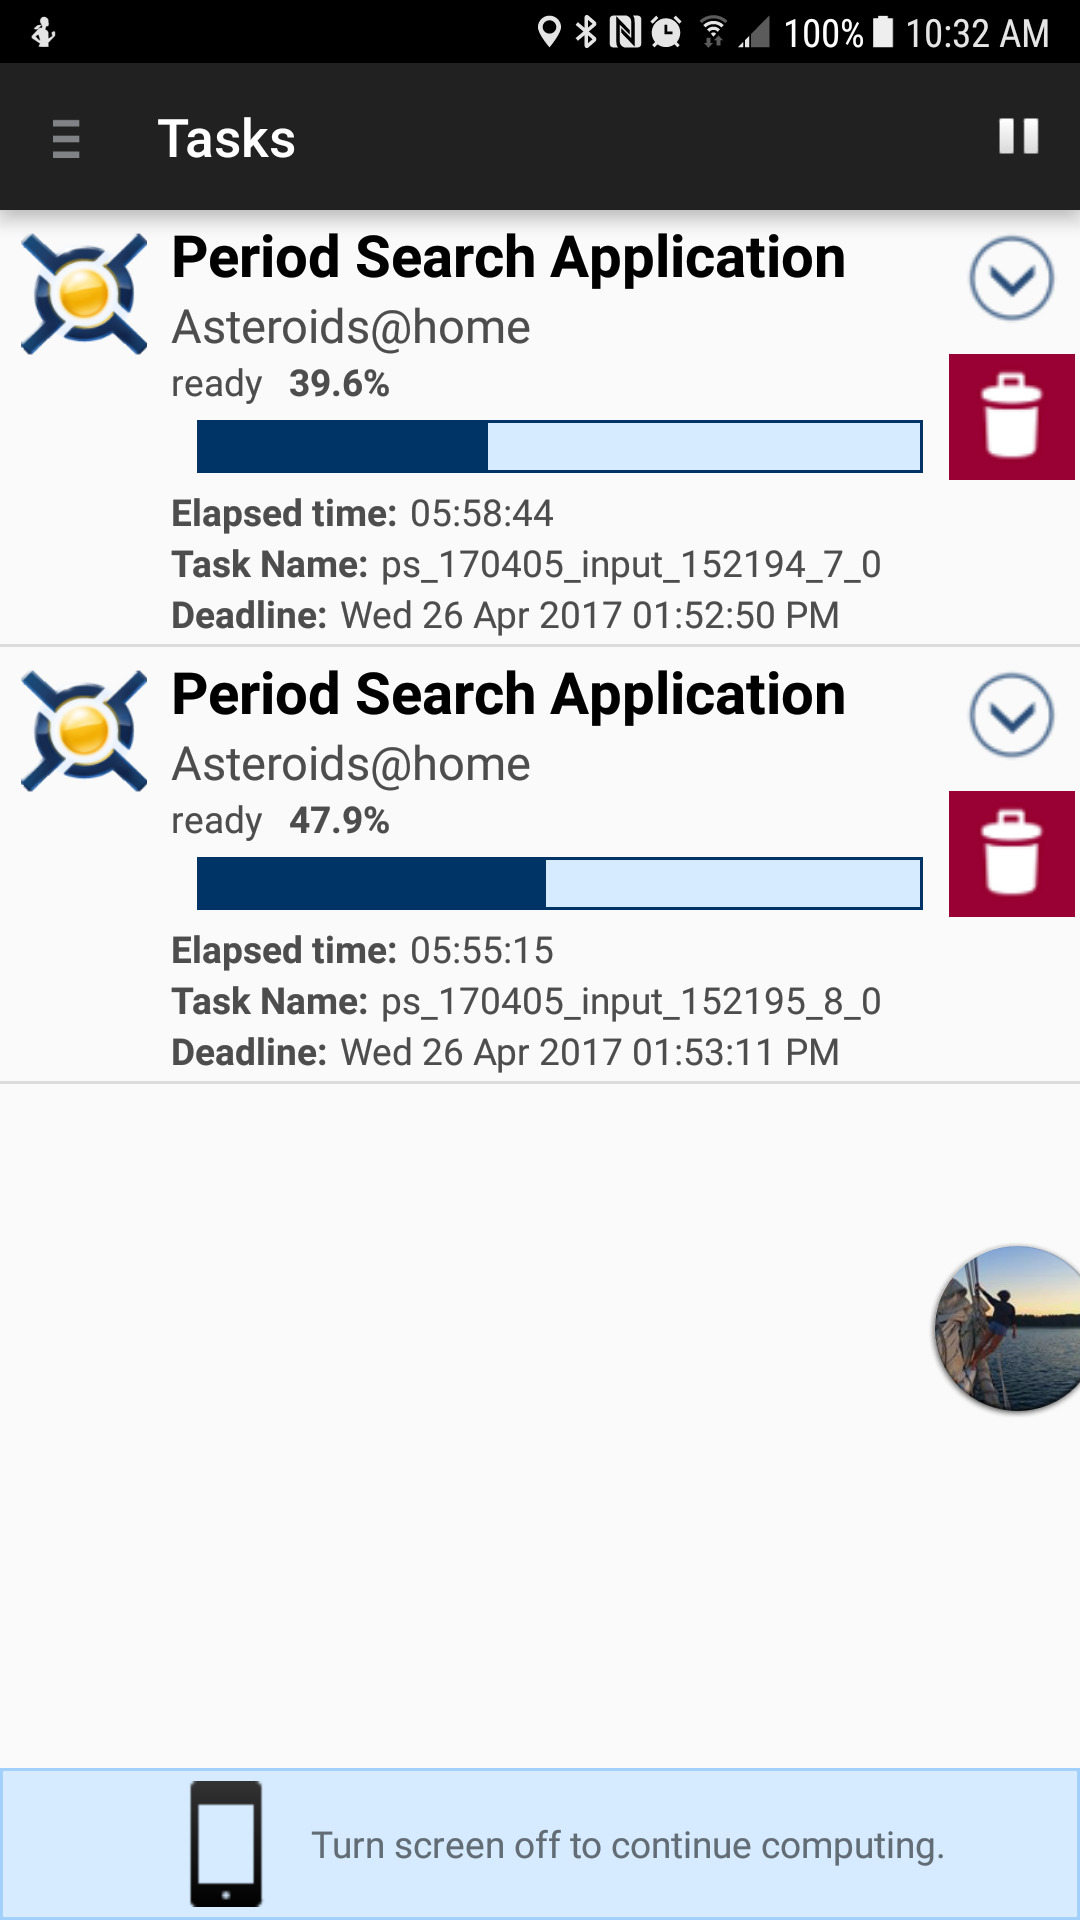
\includegraphics[width=3in]{img/t1s3.png}
      \centering
      \caption{Progress from day 1}
\end{figure}
\begin{figure}[ht]
      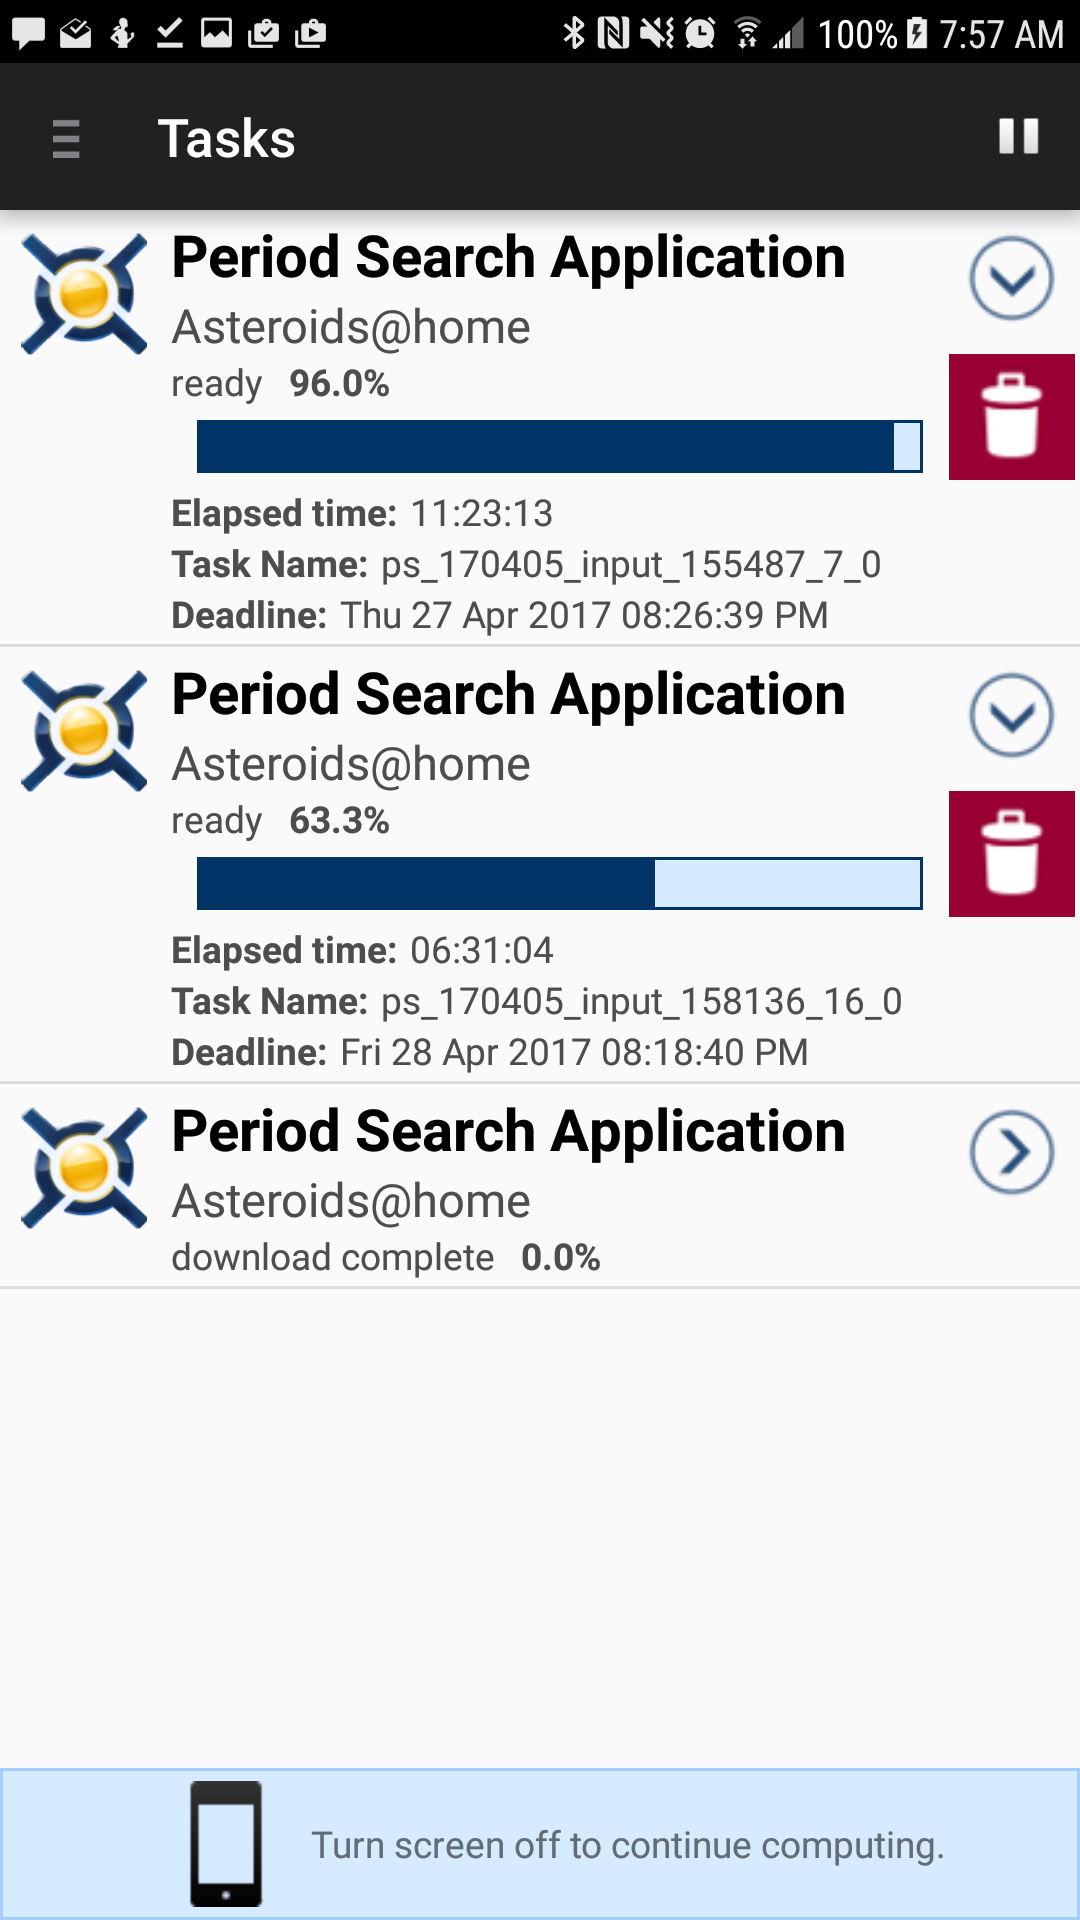
\includegraphics[width=3in]{img/t1s4.png}
      \centering
      \caption{Progress from day 2}
\end{figure}

\clearpage

\section{Task 2}
I produced a Java application that performs the operations as requested.
My solution ran very slowly the first time, but some sort of caching mechanism has significantly sped up subsequent runs.
I accomplished this by constructing a list of filenames, converting the list into pairs of CountryCode:List<File>, then map each of those into pairs of CountryCode:Average

It pulls from git into a runtime directory. It clears that directory prior to each run.

Here is some sample output
\begin{verbatim}
0963: 2.0346270892724263
0039: 2.497121913542728
0020: 2.482912862361559
0224: 2.5064794712503855
0886: 2.031443575363211
0358: 2.487213467955851
0260: 2.498950258382201
0964: 2.4859001101274973
0421: 2.0362377693372364
0359: 2.5038219030597273
0381: 2.036961360734139
0598: 2.4952199826977104
0249: 2.0439443926662517
0385: 2.4932353358828014
0048: 2.031700636922881
0995: 2.5045553311782034
0060: 2.4870613780309125
0066: 2.040048859385248
0961: 2.4906355022339746
0264: 2.4859335345521987
0380: 2.5071121604999536
0357: 2.480003068188968
0962: 2.496391443943661
0061: 2.4949891674941185
0350: 2.492618626139117
0976: 2.49331392684602
0049: 2.501967421920139
0354: 2.5108640198328085
0856: 2.4922963055148704
0046: 2.0418650963146003
0977: 2.4903605594387757
0593: 2.4877352903158974
0244: 2.510779610790489
0032: 2.5089838553833435
0685: 2.03746250587257
0218: 2.4789495459063033
0351: 2.033769082041389
0233: 2.498871601444859
0974: 2.031594345971666
0047: 2.03074610833117
0591: 2.5015689169648727
0216: 2.0382796625335007
0044: 2.493938467777325
0036: 2.4974230589053814
0213: 2.501618815735348
0030: 2.5015851501994595
0355: 2.4992061728800534
0045: 2.491333390006758
0255: 2.5101327357073293
0234: 2.0361698000628907
0001: 2.5079353295034026
0256: 2.4988984183053455
0086: 2.4839092135457226
0033: 2.4870004750328527
0967: 2.5050277577686084
0212: 2.491111047557384
0965: 2.4789036099883557
0231: 2.4989827678793834
0055: 2.498293998772541
0043: 2.492438525259559
0034: 2.0363726753047695
0251: 2.47525380382797
0254: 2.4852443085519087
0040: 2.0352504201186843
0353: 2.4979496597802036
0053: 2.481633565422152
0056: 2.5094874299856262
0084: 2.498884713203394
0373: 2.492572458044035
0090: 2.4947935304770676
0081: 2.496606897397959
0252: 2.047368990656362
0098: 2.5025838927152044
0051: 2.0341386726429245
0370: 2.4918560407668826
0052: 2.4763986206909396
0371: 2.4867651899970076
0250: 2.0360839423153667
0091: 2.5007677701785047
0092: 2.0356616705030444

Process finished with exit code 0
\end{verbatim}

The global average is quite poor.

\section{Task 3}
For task 3 I built the application and then modified actibity 1 to display little text snippets bound to an arraylist. 
I was unsure how to bind videos and stuff from the cloud - would it just be a matter of having a list of URLs or something?
If so, I feel like what i've done is basically that, but instead of setting the content source of a video object I set the content source of a text view...

\begin{figure}[ht]
      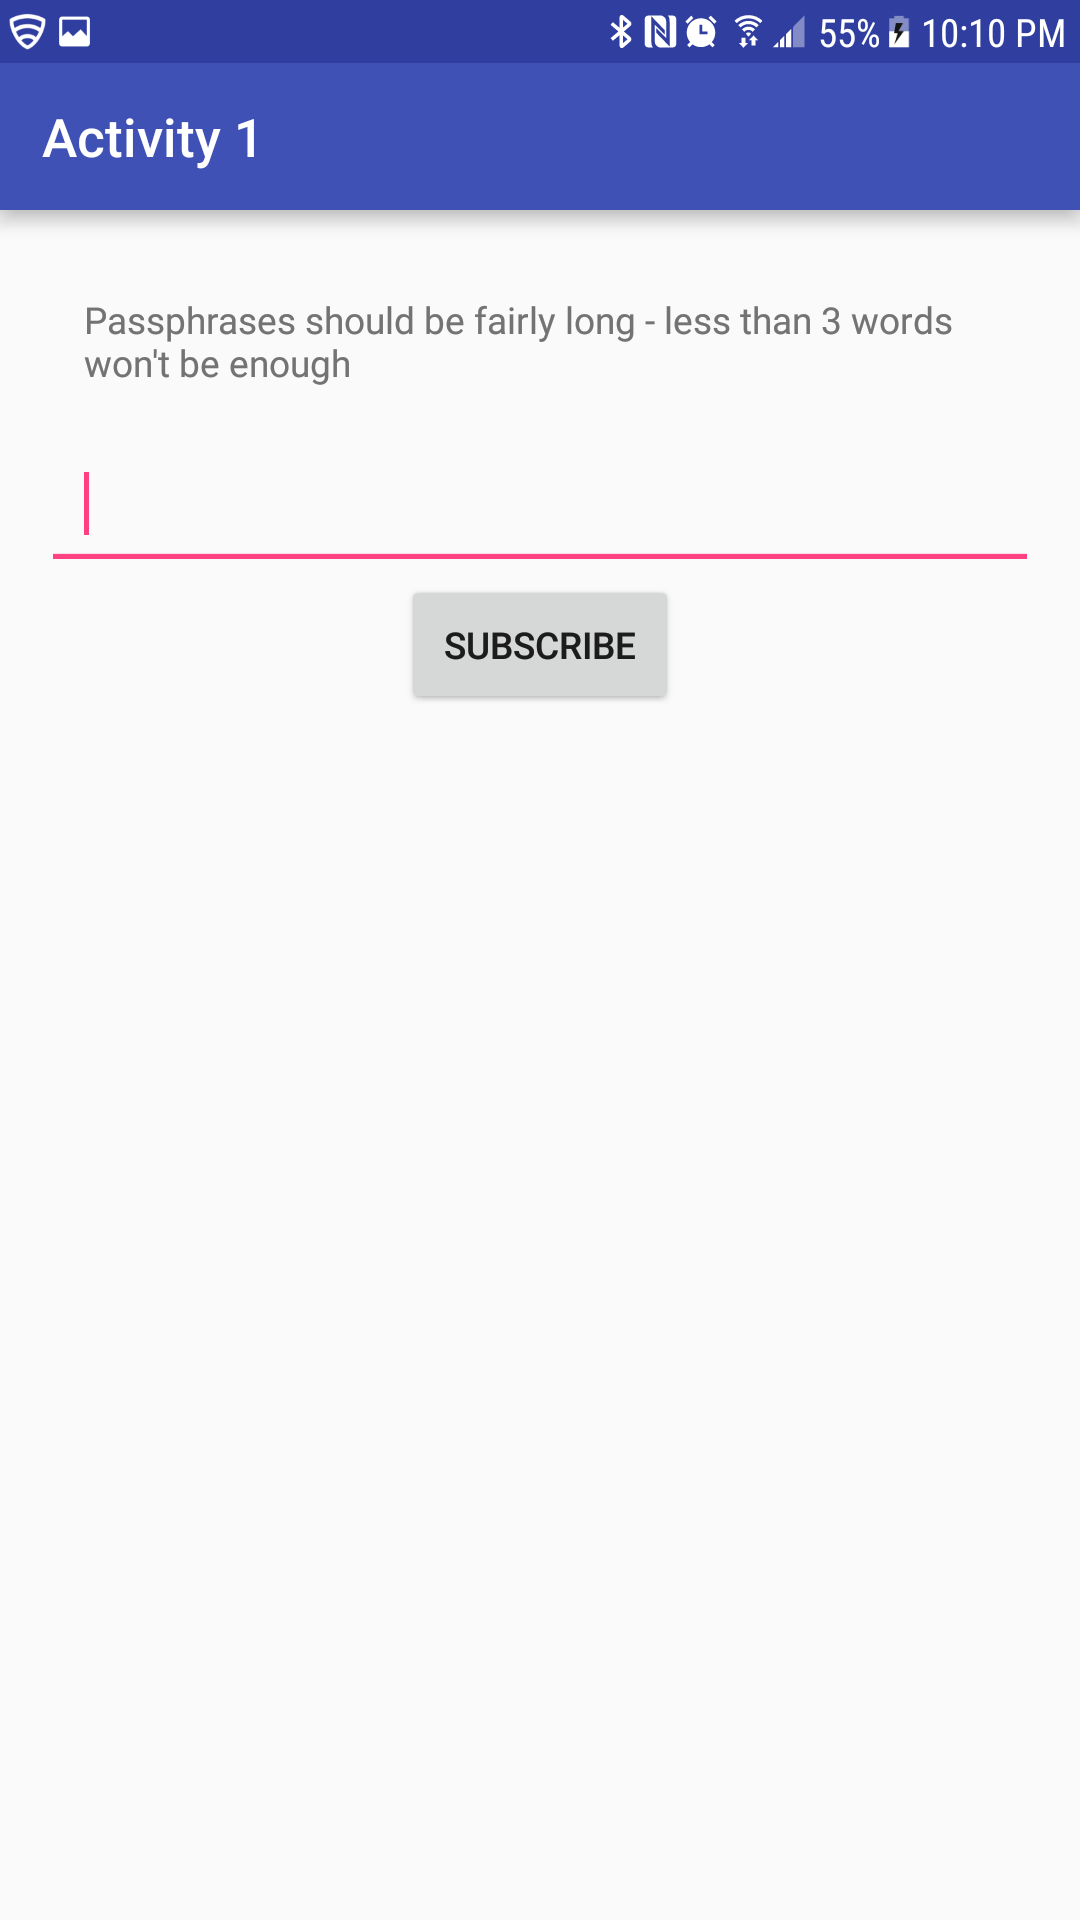
\includegraphics[width=3in]{img/t3s1.png}
      \centering
      \caption{Example 1}
\end{figure}
\begin{figure}[ht]
      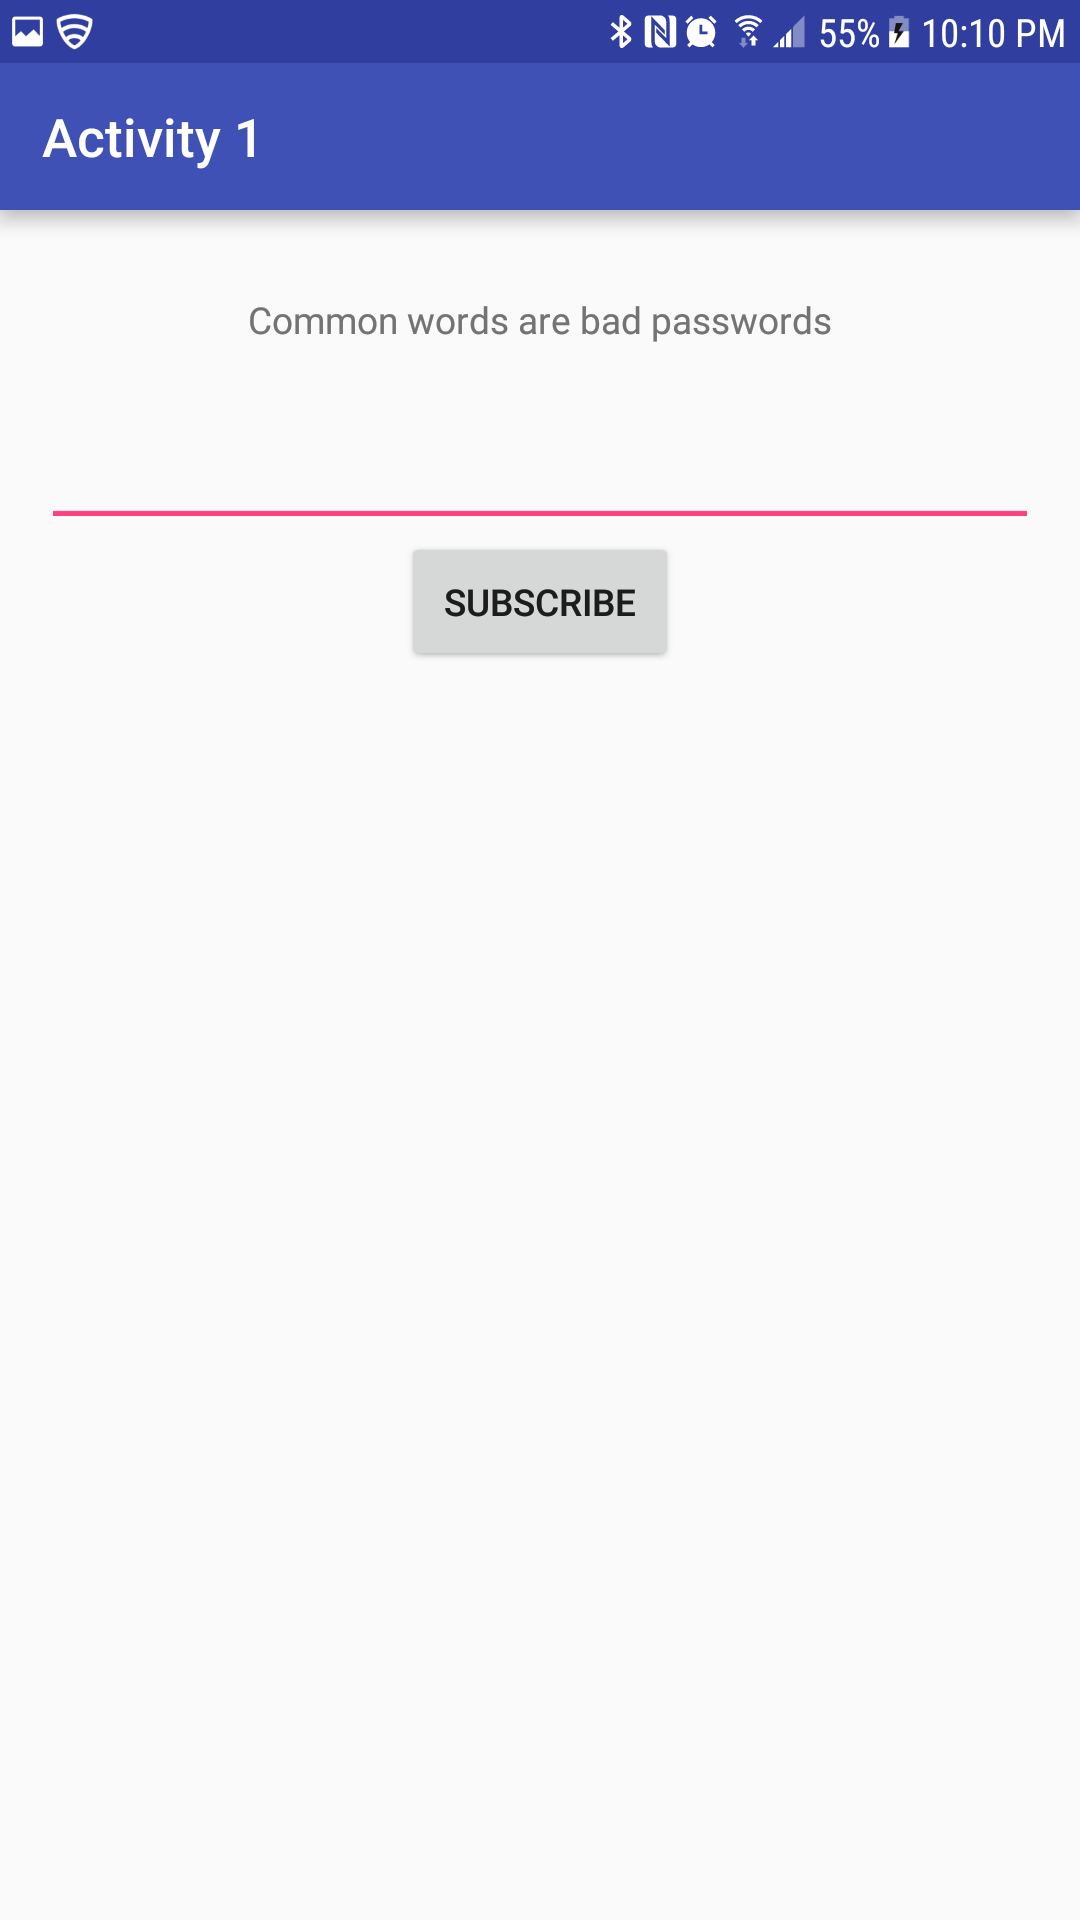
\includegraphics[width=3in]{img/t3s2.png}
      \centering
      \caption{Example 2}
\end{figure}
\begin{figure}[ht]
      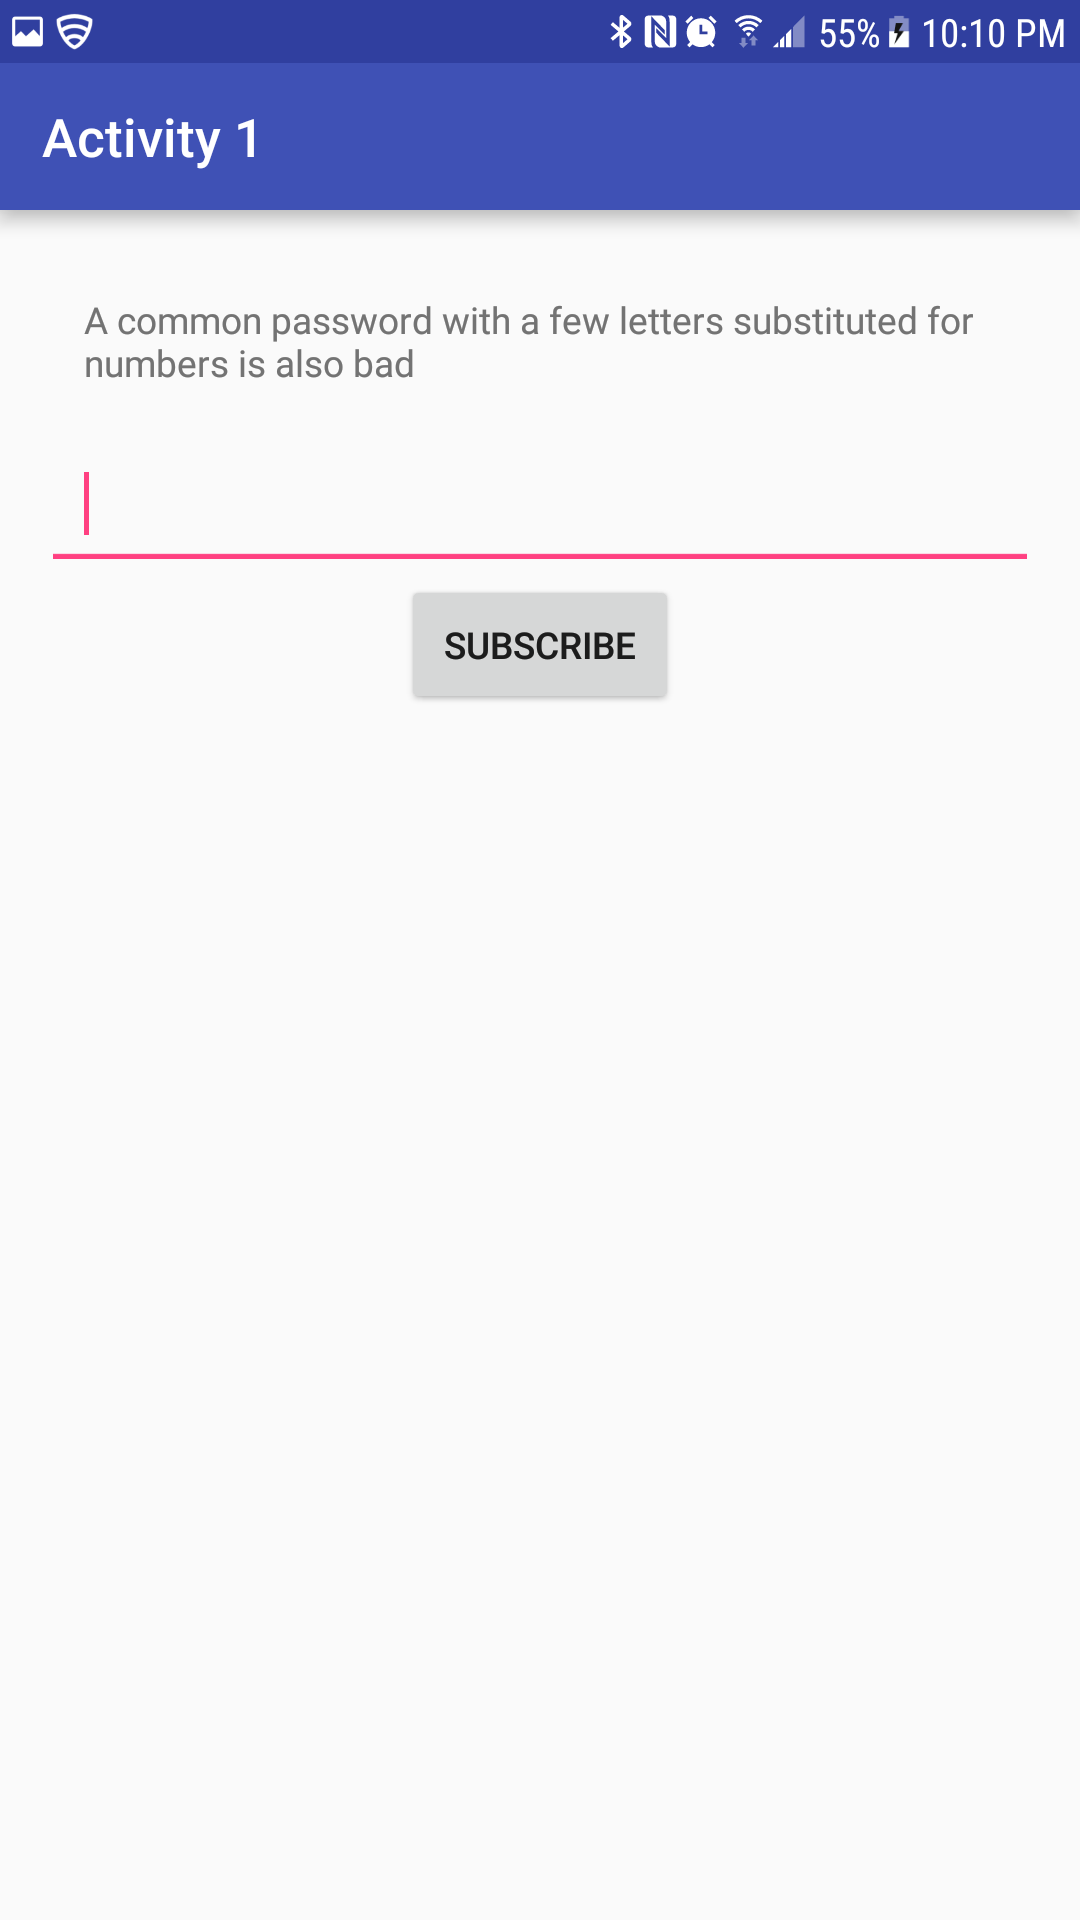
\includegraphics[width=3in]{img/t3s3.png}
      \centering
      \caption{Example 3}
\end{figure}

\clearpage
\section{Task 4}
Using Kinvey, create a bookshelf application.
Define a model for books.
The model should have the following fields: Publish date, Author (Required), Title (Required), genre, and text. See the kinvey Datastore and Data Modeling docs. 
Text should be a reference to a data file stored on the kinvey backend - see the Kinvey File API.
On the UI end, make a list of the books on the user's bookshelf, allowing them to click to view a record, or long click to delete it.
Provide an interface for adding new records.
Provide an interface for editing existing records.

Accomplish the above using the MVC design pattern - using Kinvey datastore and data modeling for the model layer.
You may wish to use the kinvey business logic model for you controller - doing so would allow you to create a REST API that your views merely query for data, however this will likely be too lengthy to implement in the required timeline without prior experience, and so is optional.

The following links should provide examples sufficinet to guide you in completing all portions of this application:
\begin{enumerate}
\item \url{https://github.com/KinveyApps/TestDrive-Android}
\item \url{https://github.com/KinveyApps/StatusShare-Android}
\end{enumerate}

\begin{figure}[ht]
      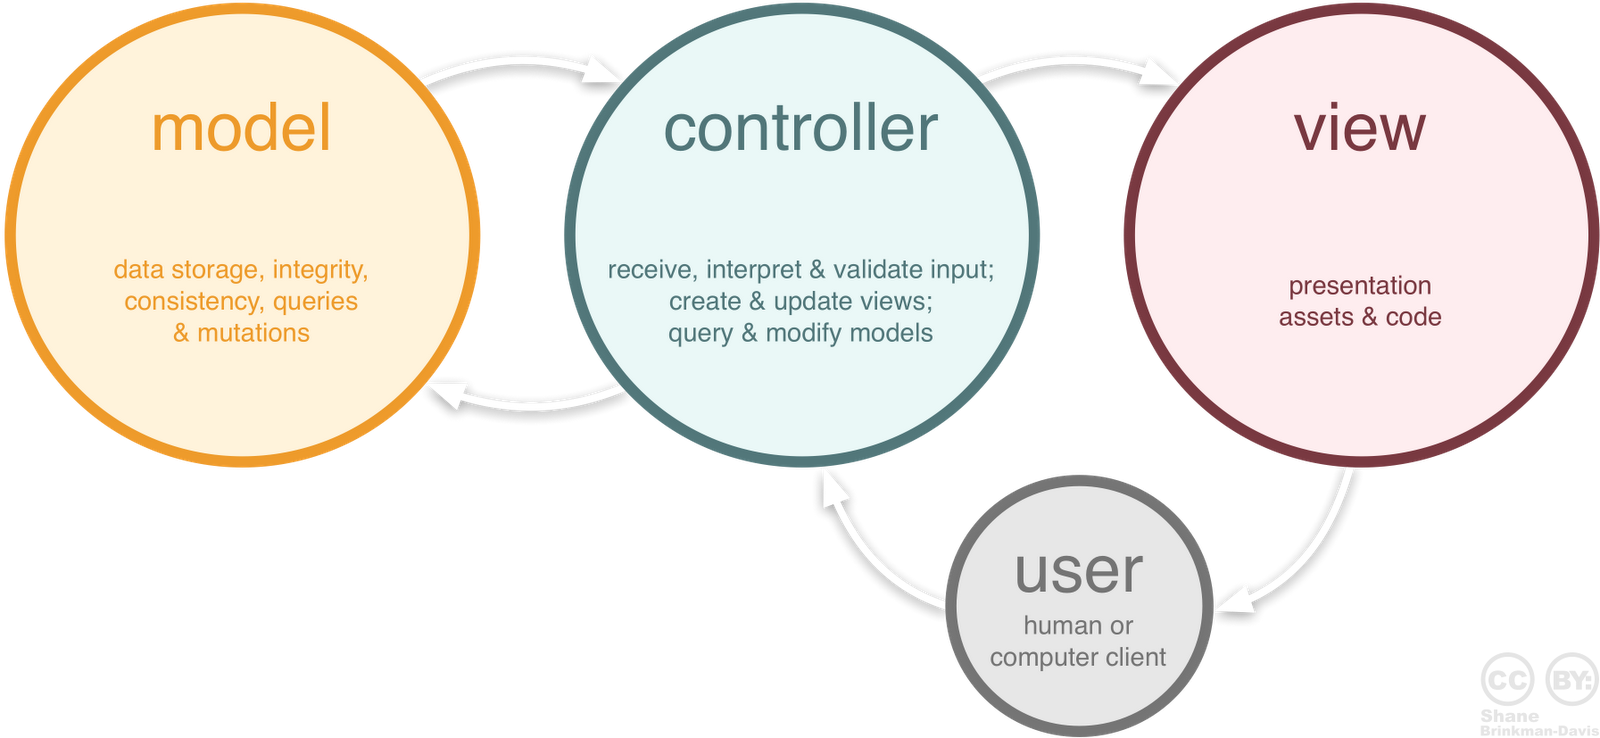
\includegraphics[width=3in]{img/mvc.png}
      \centering
      \caption{MVC diagram. Your controller, which may be on the backend, controls updating and inserting data. The models are stored on the kinvey datastore and accessed by the controller. The view is created locally in android.}
\end{figure}

\subsection{Thoughts}
I feel like this project is inherently grounded in a misnomer - MBaaS I think implies that a third party is hosting the project. As a result, there won't really be any docker containers to do this for you - the whole point of MBaaS is the "aaS": you're paying someone else to host your mobile backend. I designed this project against Kinsey a powerful mobile backend with a robust api and lots of documentation. I don't think you'll find any dockers (I certainly couldn't) that provide functionality even close to this - it's a very complex system, and that's why you're hiring someone else to do it for you, and even if it was as simple as firing up a docker container, I think such a system would scale very very poorly (and defeat the point of "aaS").

\clearpage

\section{Task 5}
To complete this portion I used a part of my previous submissions for running SSH, which means that remote crack tests require root.
That said, it does seem to work just fine otherwise.

To create passphrases, I read in a list of the 5000 most common english words. I then stitch together 7 of them, selected at random, to form a single password. I place this text in the edit bar for ease of use, and so that the user can test the passphrase strength.

For the cracking portion, I run the password through md5sum and pipe the result into hashcat running on mode 0 attack 0. I push the output to the text field.

You can see this all in action here:
\begin{figure}[ht]
      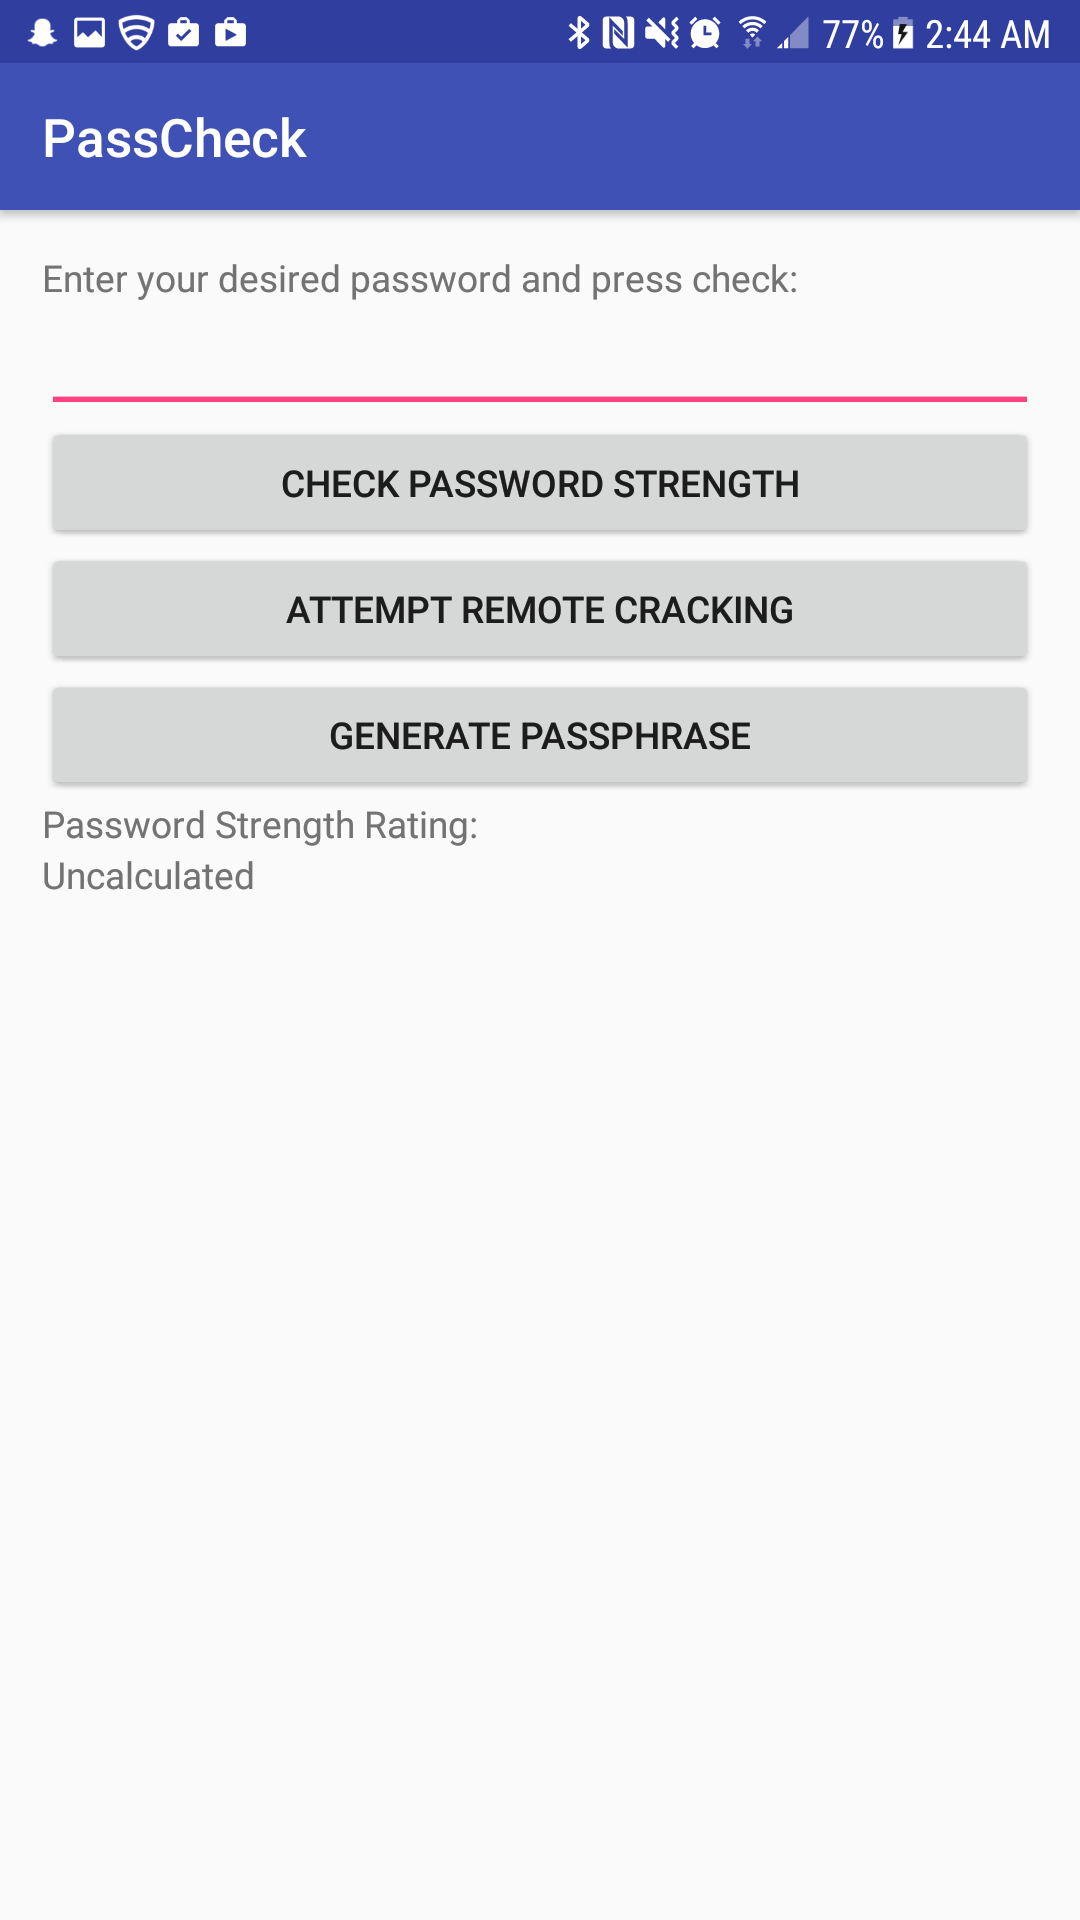
\includegraphics[width=3in]{img/t5s1.png}
      \centering
      \caption{Base Screen}
\end{figure}
\begin{figure}[ht]
      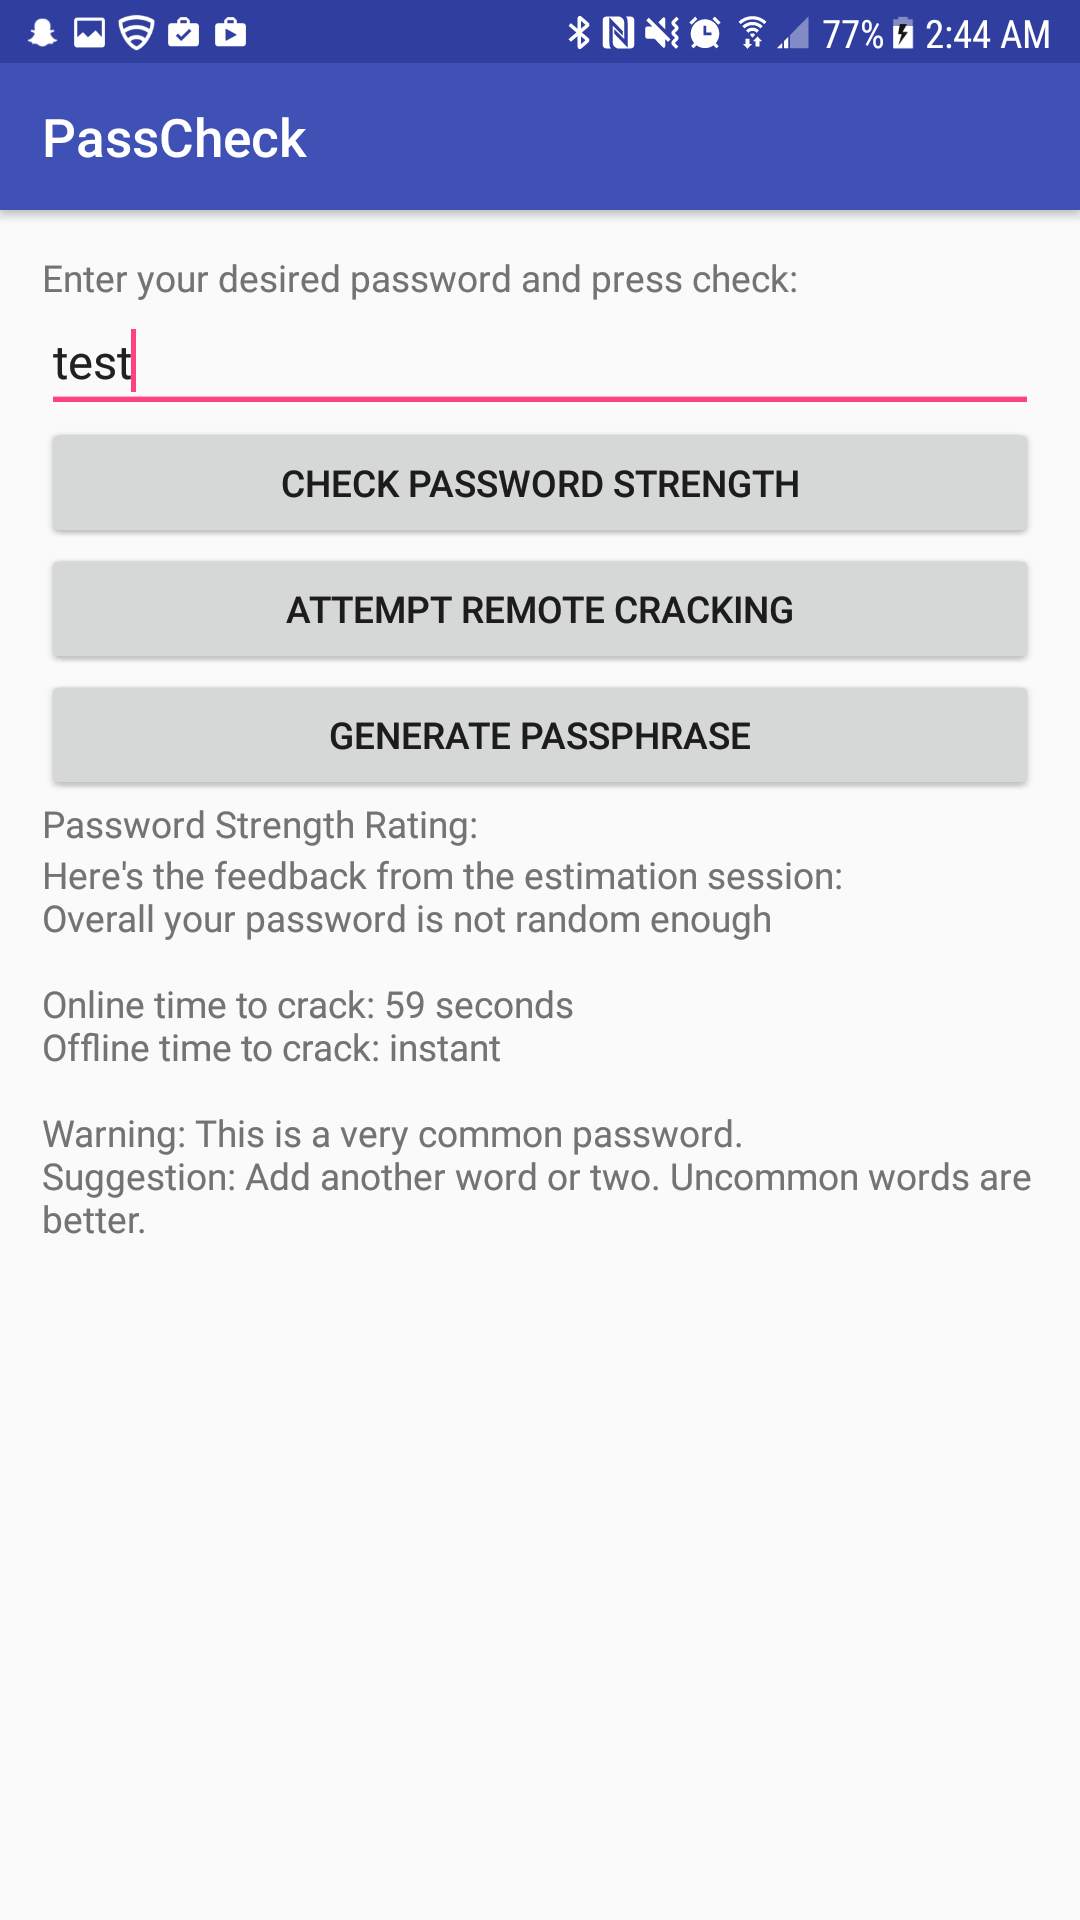
\includegraphics[width=3in]{img/t5s2.png}
      \centering
	\caption{Demo of a weak password (same functionality as before)}
\end{figure}
\begin{figure}[ht]
      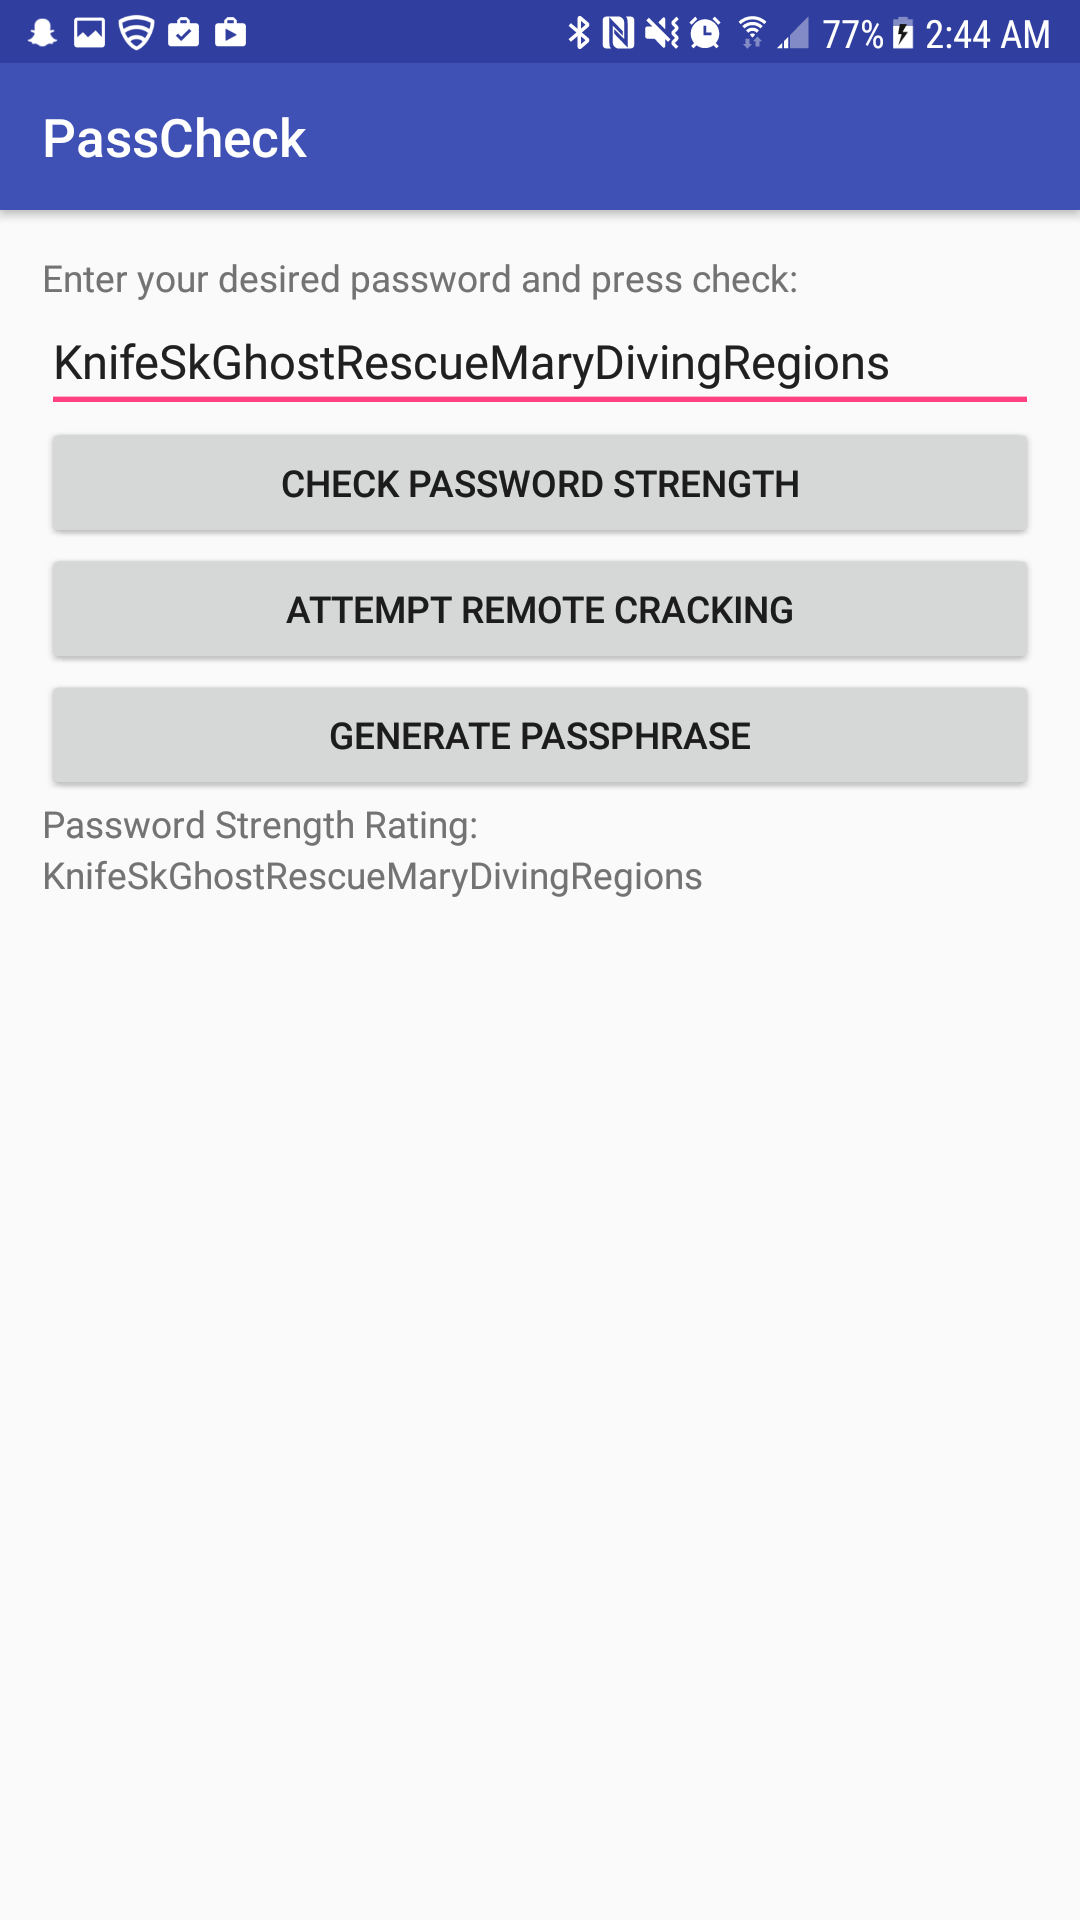
\includegraphics[width=3in]{img/t5s3.png}
      \centering
      \caption{Generated password}
\end{figure}
\begin{figure}[ht]
      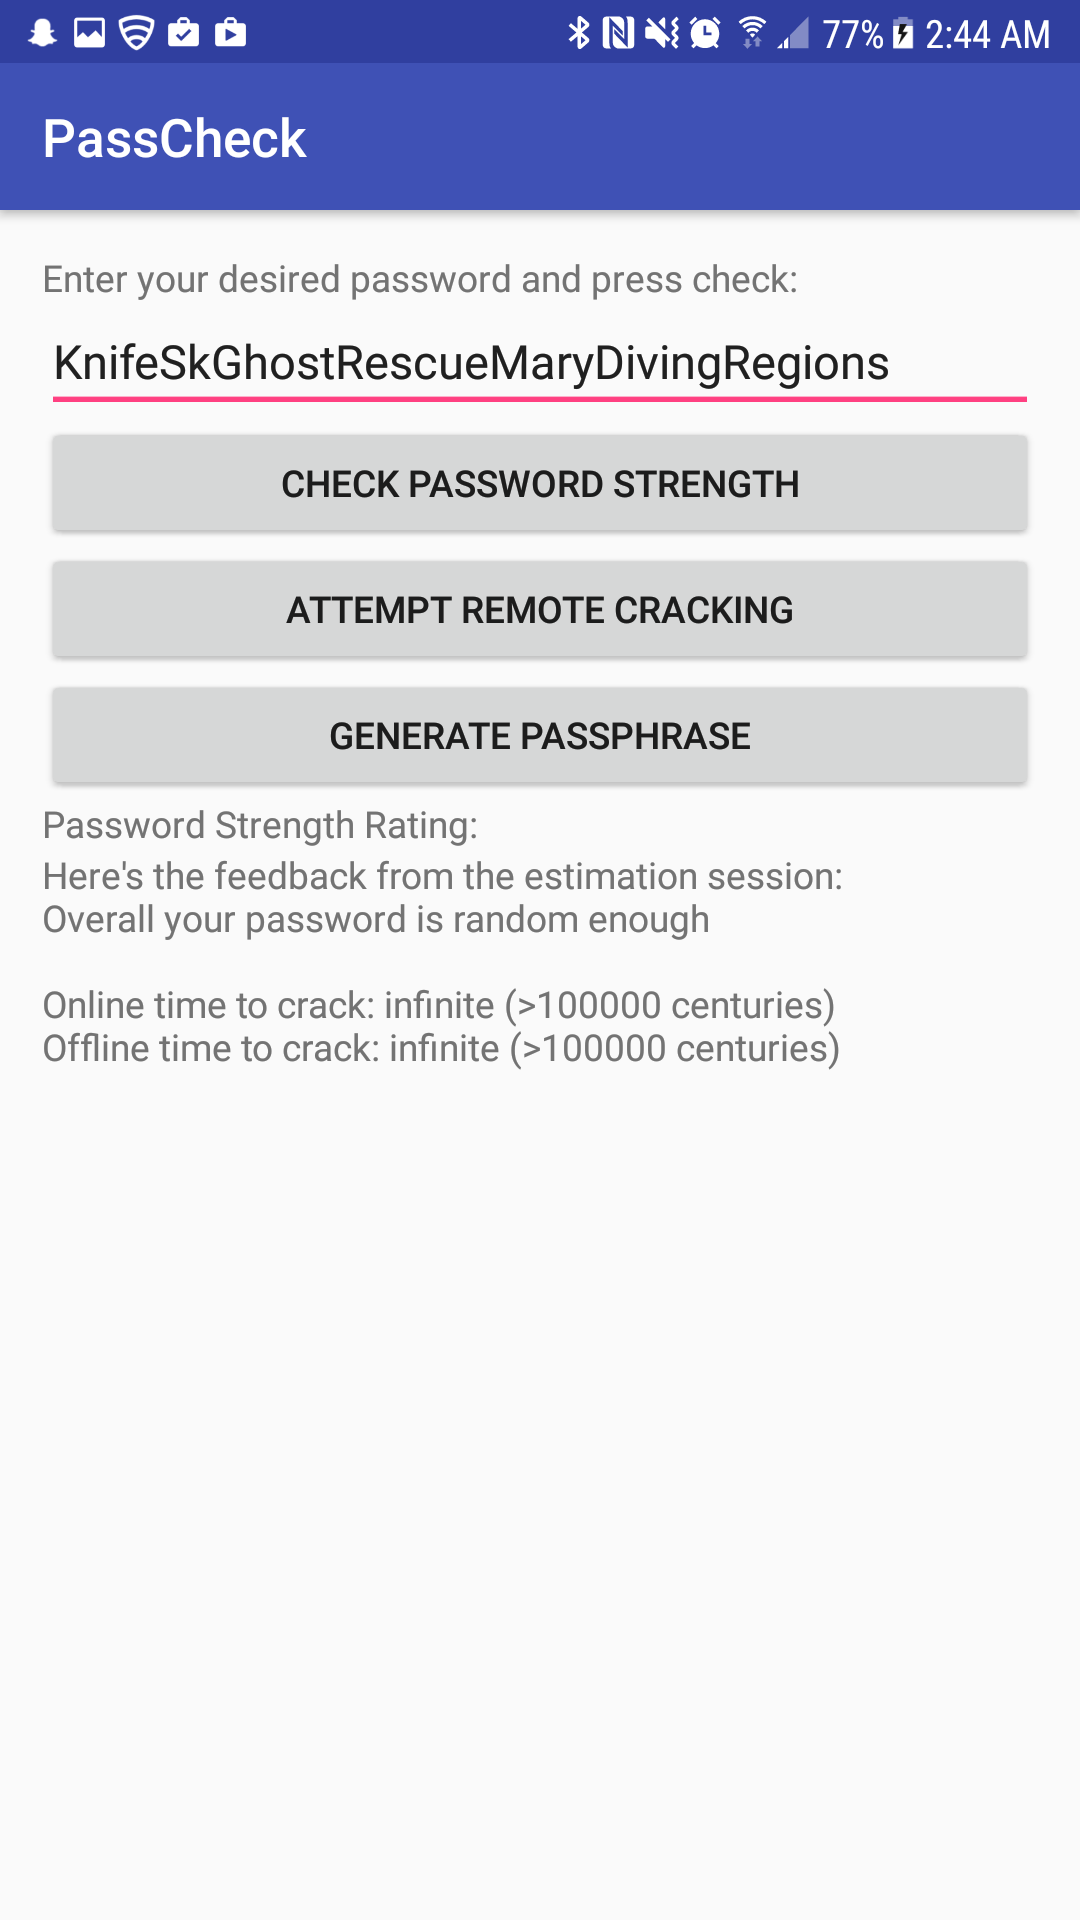
\includegraphics[width=3in]{img/t5s4.png}
      \centering
      \caption{Generated password strength test}
\end{figure}

\clearpage

\end{document}
